\section{Iteration \#0 -- Evaluation Framework and Baselines}

This iteration built for an evaluation framework that streamlined the evaluation process and discusses the implementations of the two evaluation baselines, Sequential Scan and Octree.

\subsection{Evaluation Framework}

Evaluation is a major part of the project and is performed multiple times at different stages of the project. It was decided a framework should be used to streamline this process and reduce the time it takes to generate the measurements required for evaluation.  The framework was created because performance analysis would be done very frequently, multiple times per iteration. Manually timing and profiling the code each time is time-consuming and error-prone. Putting more effort initially into creating a system that allows large sets of operations and index structures to be tested at once may save a significant amount of time, especially as many of these performance test are long and must be run multiple times to get average times. No tool for this specific task existed, so one was created fpr this project.

The evaluation framework takes a specification containing all the datasets and index structures to test, and executes the Insert-Query-Delete operation list for the given datasets on all specified structures. The output is a set of text files containing the performance measures described in Section \ref{sec:performance-measures}. The text files the executable produces are fed into Python scripts to automatically generate tables and plots.

There are three core modules of the framework, which are shown in Figure \ref{fig:evaluation-framework} and listed below:
\begin{itemize}
	\item \texttt{data} -- library that contains standard data types used throughout framework and index structures, as well as dataset generators/loaders
	\item \texttt{index\_structure} -- library that contains every index structure implemented in the project
	\item \texttt{evaluator} -- executable program that takes specification file and runs a set of automated performance tests to produce text files containing evaluation measures
\end{itemize}

\begin{figure}
	\centering
	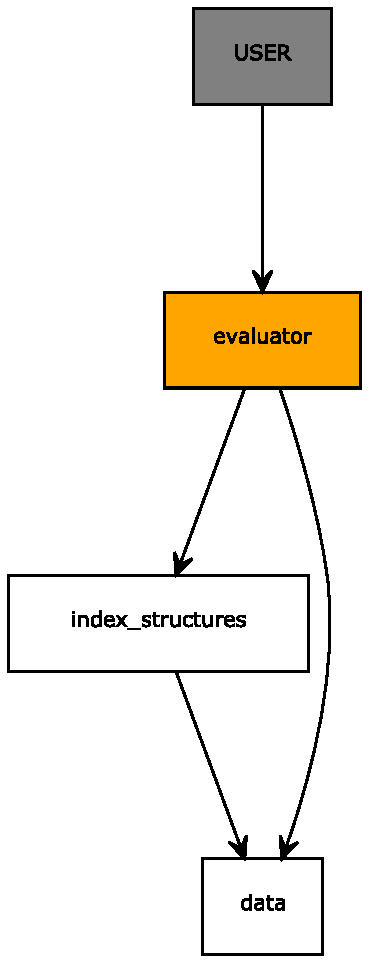
\includegraphics[scale=0.6]{figures/evaluation_framework.pdf}
	\caption{Modules of Evaluation Framework}
	\label{fig:evaluation-framework}
\end{figure}

\subsection{Baseline Implementations}
 
Sequential scan was implemented using the C++ container \texttt{std::vector}, a dynamically resizeable array.  Point queries are performed in $O(n)$ time, as the query iterates through the array sequentially until the given point is found or the end of the array is reached. The structure must check if a point exists in the structure before inserting it, making \texttt{insert} take $O(n)$. \texttt{delete} is a standard array deletion, making it an $O(n)$ operation.

The octree variant implemented is a bucket PR octree. The structure partitions the underlying data space into uniformly sized boxes, without using the points as pivots (unlike point quadtrees). It is a bucket octree because \textit{multiple} points can be stored in a single leaf node. The octree dynamically decomposes spatial regions based on its current contents. When the number of points in a leaf node exceeds a certain number, say $M$, then the region represented by the leaf is sub-divided, creating $2^d$ children. The $M + 1$ points are then scattered across the children. Therefore, dense regions of space have a finer decomposition than sparse regions.

When a point is deleted from a leaf, the leaf's contents and its siblings are checked. If all of these nodes are empty, they are removed and the sub-regions are collapsed into a single node representing the whole region. If the collapsed node and its siblings are empty, then they are collapsed into their parent. This is repeated until there is a parent whose children contain at least one point.

\subsection{Compiler Optimisation}

GCC\footnote{GCC, the GNU Compiler Collection -- \url{http://gcc.gnu.org/}} was the C++ compiler used in this project. GCC can automatically modify the compiled program to make it more efficient on the target platform. There are multiple optimisation levels, going from 0 (no optimisation) to 3 (maximum optimisation). In order to make the structures as fast as possible, level 3 optimisation was used to compile the structures.

Table \ref{tab:compiler-optimisation} shows the execution times of the two baselines on 10,000 random 10D points, when level 0 and level 3 optimisation is used. Level 3 optimisation consistently sped up the structures, showing that the potential speed gains are huge. For example, the octree's point queries are approximately $6.5$ times faster, just by enabling level 3 optimisation. Level 3 optimisation will be used when compiling all index structures in the project.

\begin{table}
	\centering
	\begin{tabular}{|l|l|l|l|}
		\hline
		\textbf{Structure} & \textbf{Operation} & \textbf{Level 0} & \textbf{Level 3} \\
		\hline
		\multirow{ 4}{*}{Sequential Scan} & Insert & 1.33509 & 0.111372 \\
		 & Delete & 5.29548 & 0.623759 \\
		 & Point Query & 1.33468 & 0.111909 \\
		\hline
		\multirow{ 4}{*}{Octree} & Insert & 1.23108 & 0.243256 \\
		 & Delete & 0.73156 & 0.13589 \\
		 & Point Query & 0.559736 & 0.0860926 \\
		 \hline
	\end{tabular}
	\caption{Total Execution Time (in Seconds) of Structure Operations With Different Levels of Compiler Optimisations (10,000 10D Random Points)}
	\label{tab:compiler-optimisation}
\end{table}